\documentclass{article}
\usepackage[utf8]{inputenc}
\usepackage{graphicx} % Allows including images
\usepackage{subcaption}
\usepackage{amsmath}

\title{Weekly Report}
\author{Junior Team }
\date{July 2020}

\begin{document}

\maketitle

\section{Assumptions and Variable Set-Up}
In order to analyze the square data set, we had to make some assumptions in order to account for some differences between the square and ellipse data sets. When we initially used the square data, we were implementing the Wang-Mason model, which we found that mass is arbitrary, since it cancels out. We figured that this is not the case for IRB Bound and assume that the square and ellipse are made of the same material to use this conversion: 

\begin{equation}
    m_{square} = m_{ellipse} * \frac{A_{square}}{A_{ellipse}}
\end{equation}

\noindent Additionally, whereas the ellipse data that we received came with the Jacobian and pre- and post-impact states, we needed to isolate these ourselves. To compute the $n$ and $d$ vectors for the Jacobian, we first identified the impact to extrapolate. From then on, we used the pre-impact data for our calculations. We then found the coordinates of all four edges of the square. We took the coordinate with the lowest $y$ value and its corresponding $x$ to be the contact point of the square. After subtracting this $(x, y)$ pairing from the COM coordinates to get the moment arms--measured from the contact point-- we put these into the third columns of the vectors. 

\begin{equation}
n = 
\begin{bmatrix} 
 0 \\
 1 \\
 x_{COM}-x_{contact} 
\end{bmatrix}
\end{equation}

\begin{equation}
d = 
\begin{bmatrix} 
 1 \\
 0 \\
 y_{COM}-y_{contact} 
\end{bmatrix}
\end{equation}

\section{Constructing Square Data Set}
This week we created an impact data set from the square trajectory files. To identify when an impact occurs, the code looks for a sign change in the vertical velocity (negative to positive) and the y coordinate of the COM must be lower than the previous and following y com position. To avoid "bad data" (double impacts, skipped frames etc...) we used our visualizer and manually recorded only the impacts that were clear (just considering the first two collisions from each drop). From 500 csv files, (1000 total potential impacts) we ended up with around 375 clear impacts. \\

\noindent The data set could be expanded, but we would need much more robust code or spend some more man-hours going through the data set in detail. With our code, if the first impact is fishy and looks like a double hit we automatically can't take data from a later impact because of the inconsistencies of the automated impact data extraction (described above w/ the y velocity/position). For now, we thought we have plenty of data points. A clear bias with the data collection however is natural clumping of pre-impact angles. When the angles are around $0$ or $\pm \frac{\pi}{2}$ a double hit is far more likely to occur so we have have far fewer data points around these impacts which are quite common because the 1/250 second data collection rate isn't quite fast enough to capture these "double hits". 

 \begin{figure}[h!]
        \centering
        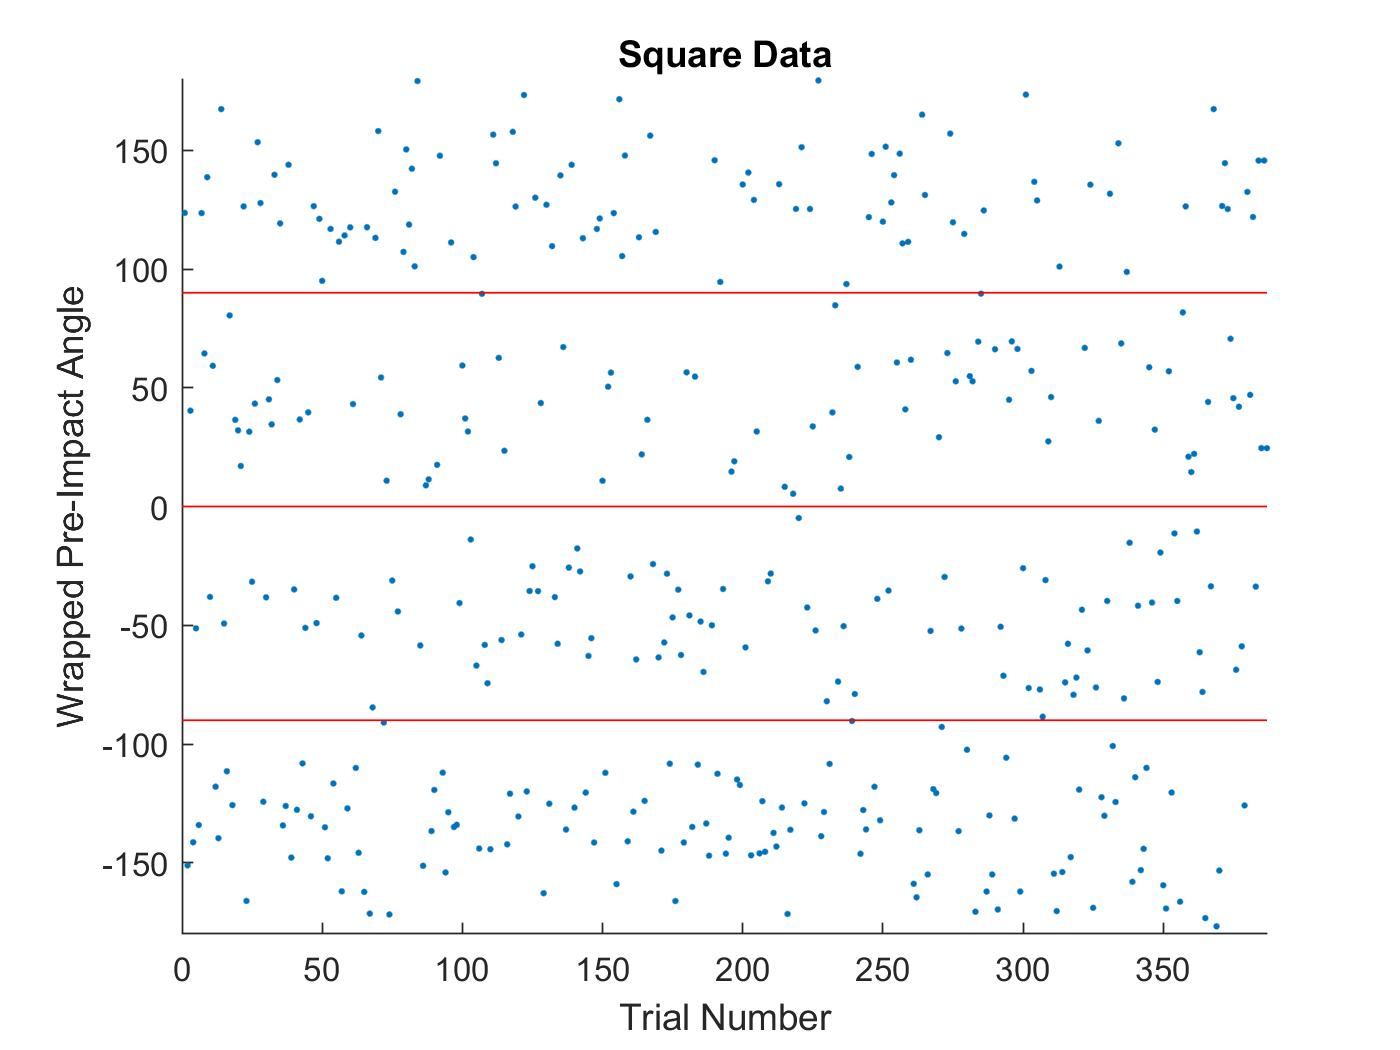
\includegraphics[scale=0.11]{SquareDataBias.jpg}
        \caption{Bias in Data Collection (Pre Impact Angle)}
        \label{fig:dataBias}
\end{figure}

\section{Comparing Ellipse  and Square Data}
\subsection{IRB with Width}
For the square, it is less intuitive to explain the error in the IRB with some sort of moment due to a contact patch width since the impacts are almost exclusively occurring at the corners. That being said, you could still use the idea behind using width as a correction factor for inaccuracies in the data collection method. 

\begin{figure}[h!]
    \centering
    \begin{subfigure}[b]{0.45\linewidth}
        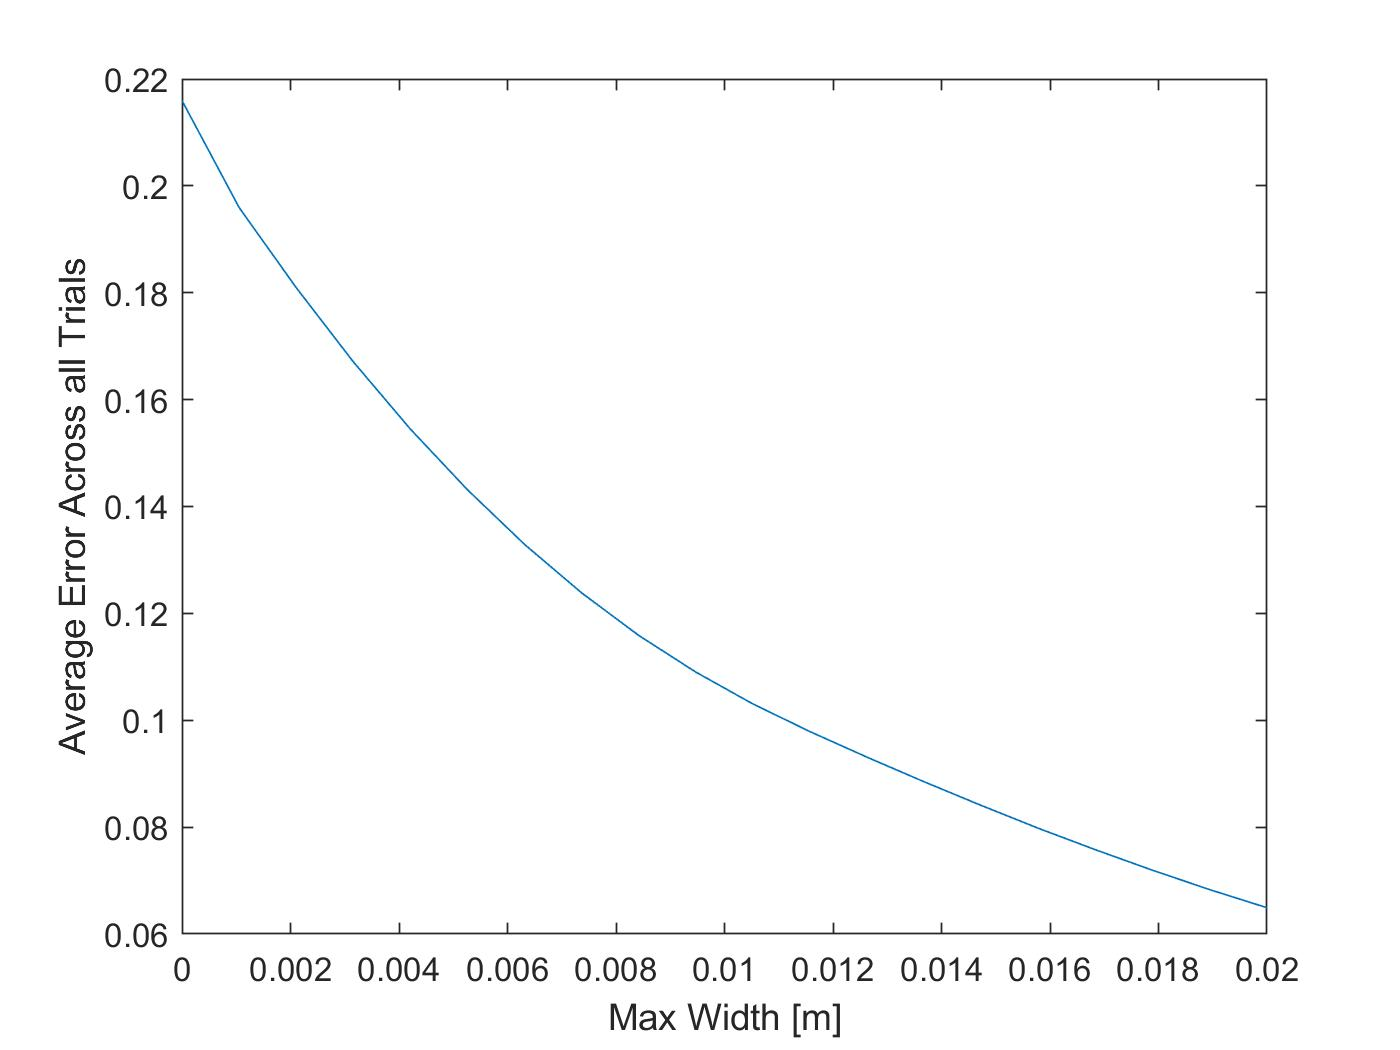
\includegraphics[scale=0.125]{squareWidth.jpg}
        \caption{Square Data Set}
        \label{fig:squareWidth}
    \end{subfigure}
    \quad
    \begin{subfigure}[b]{0.45\linewidth}
       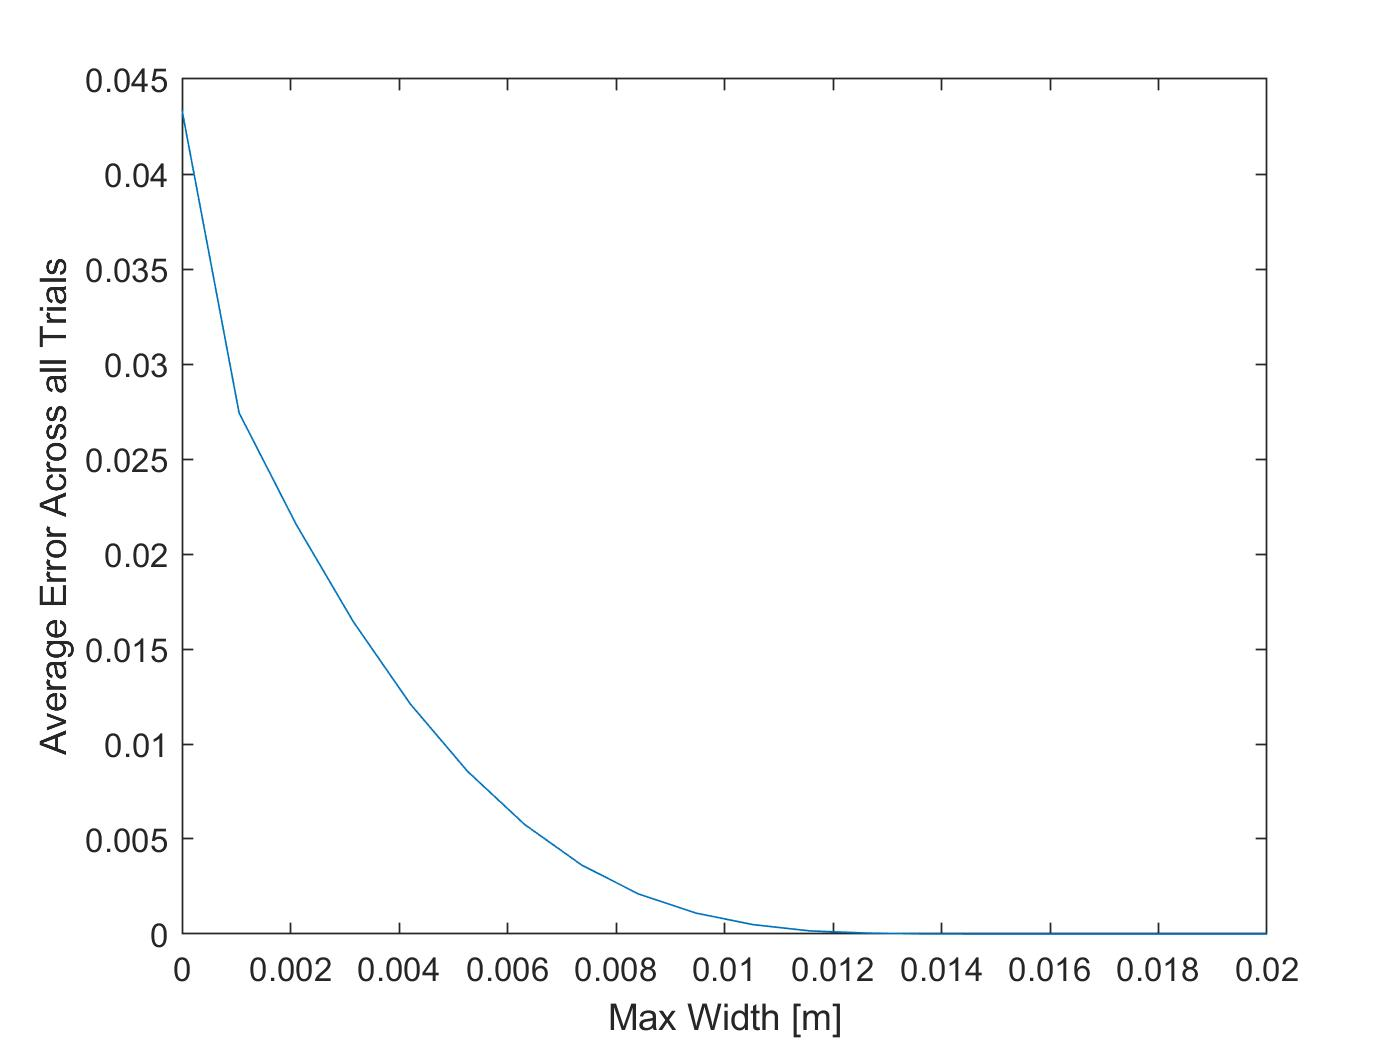
\includegraphics[scale=0.125]{ellipseWidth.jpg}
        \caption{Ellipse Data Set}
        \label{fig:ellipseWidth}
    \end{subfigure}
    \caption{Error from IRB model over range of max widths}
\end{figure}

\noindent Although adding the width correction factor does lower error, the overall magnitude of errors for the square data is still much larger then that from the ellipse data set. Even at a width of 2cm (largest in max widths tested) the average error from the square is around twice as large as the average error from the ellipse data set with no width (max width = 0). The curve is also sloped much more steeply, showing larger decreases in error and ending at basically 0 average error for the ellipse set. Another interesting point is that when the max width is set to 2cm for the ellipse data set (unrealistically large) all trials have an optimal width below this cap. For the square data set however, tons of trials clump at the bounds of this unrealistic cap (\ref{fig:squareAngleWidth}) meaning a larger magnitude width would decrease error. It seems as though the classical IRB model is far worse at predicting the square impacts and width is not a natural correction factor. 

\subsection{Pre Impact Angle vs. Width}
With the ellipse data set, we were seeing a sinusoidal relationship between the pre-impact angle of the ellipse and the optimal width (which can also be interpreted as error) from the IRB model (with width). This same trend doesn't seem to arise from the square data set.  This could be due to ideas from Fig \ref{fig:dataBias} (bias in the data set), ideas from section 3.1, or a combination of both.   

\begin{figure}[h!]
    \centering
    \begin{subfigure}[b]{0.45\linewidth}
        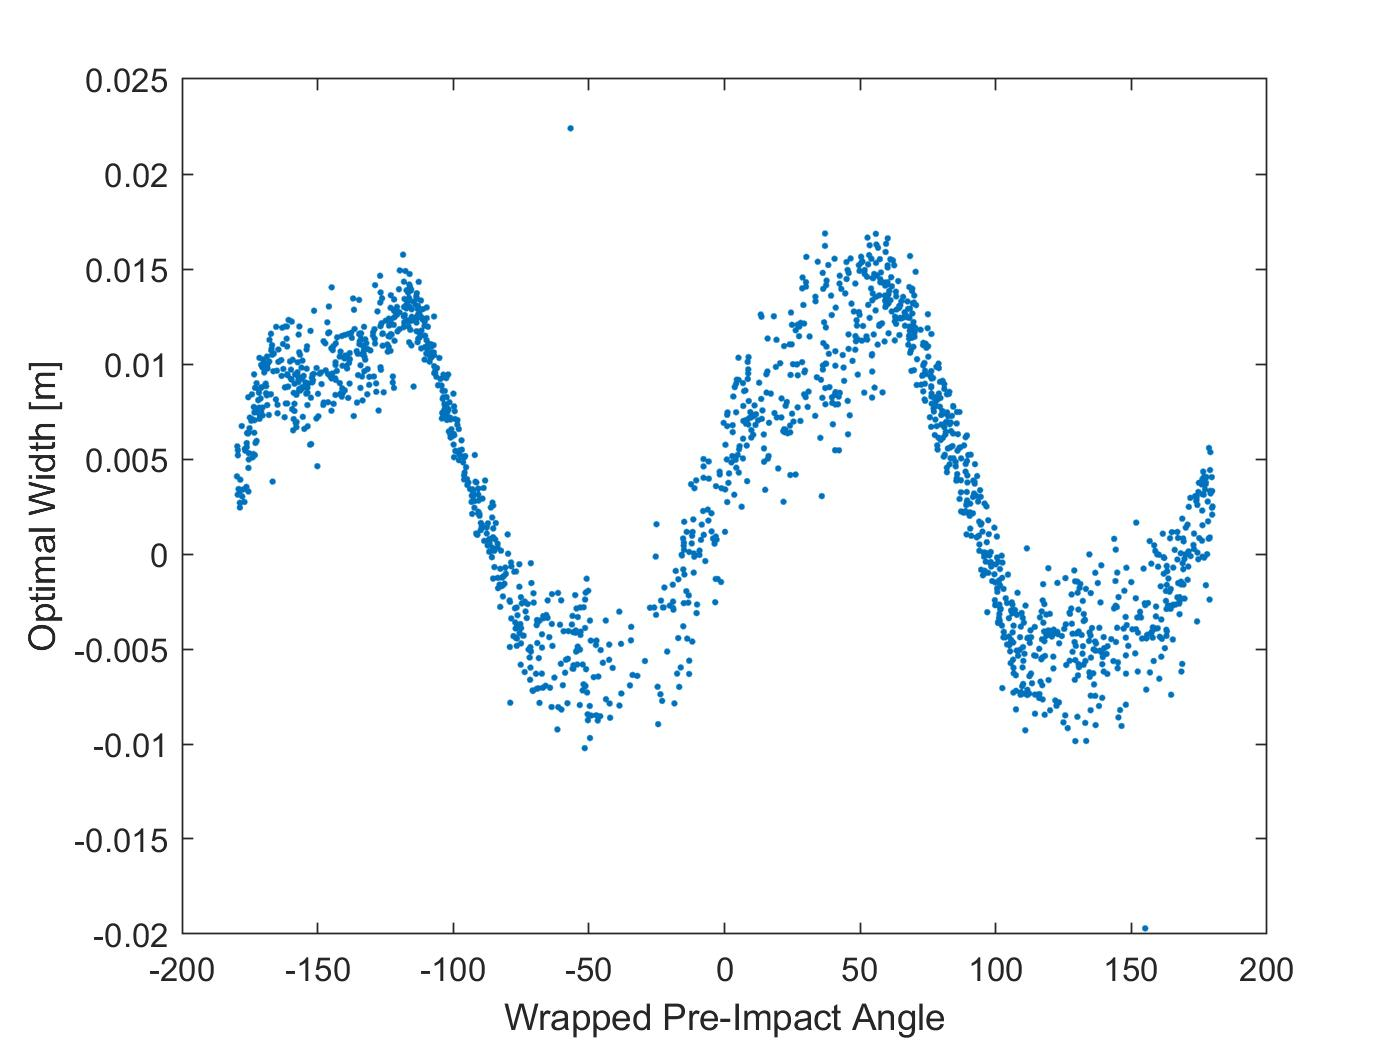
\includegraphics[scale=0.125]{ellipseAngleWidth.jpg}
        \caption{Ellipse Data Set}
        \label{fig:ellipseAngleWidth}
    \end{subfigure}
    \quad
    \begin{subfigure}[b]{0.45\linewidth}
       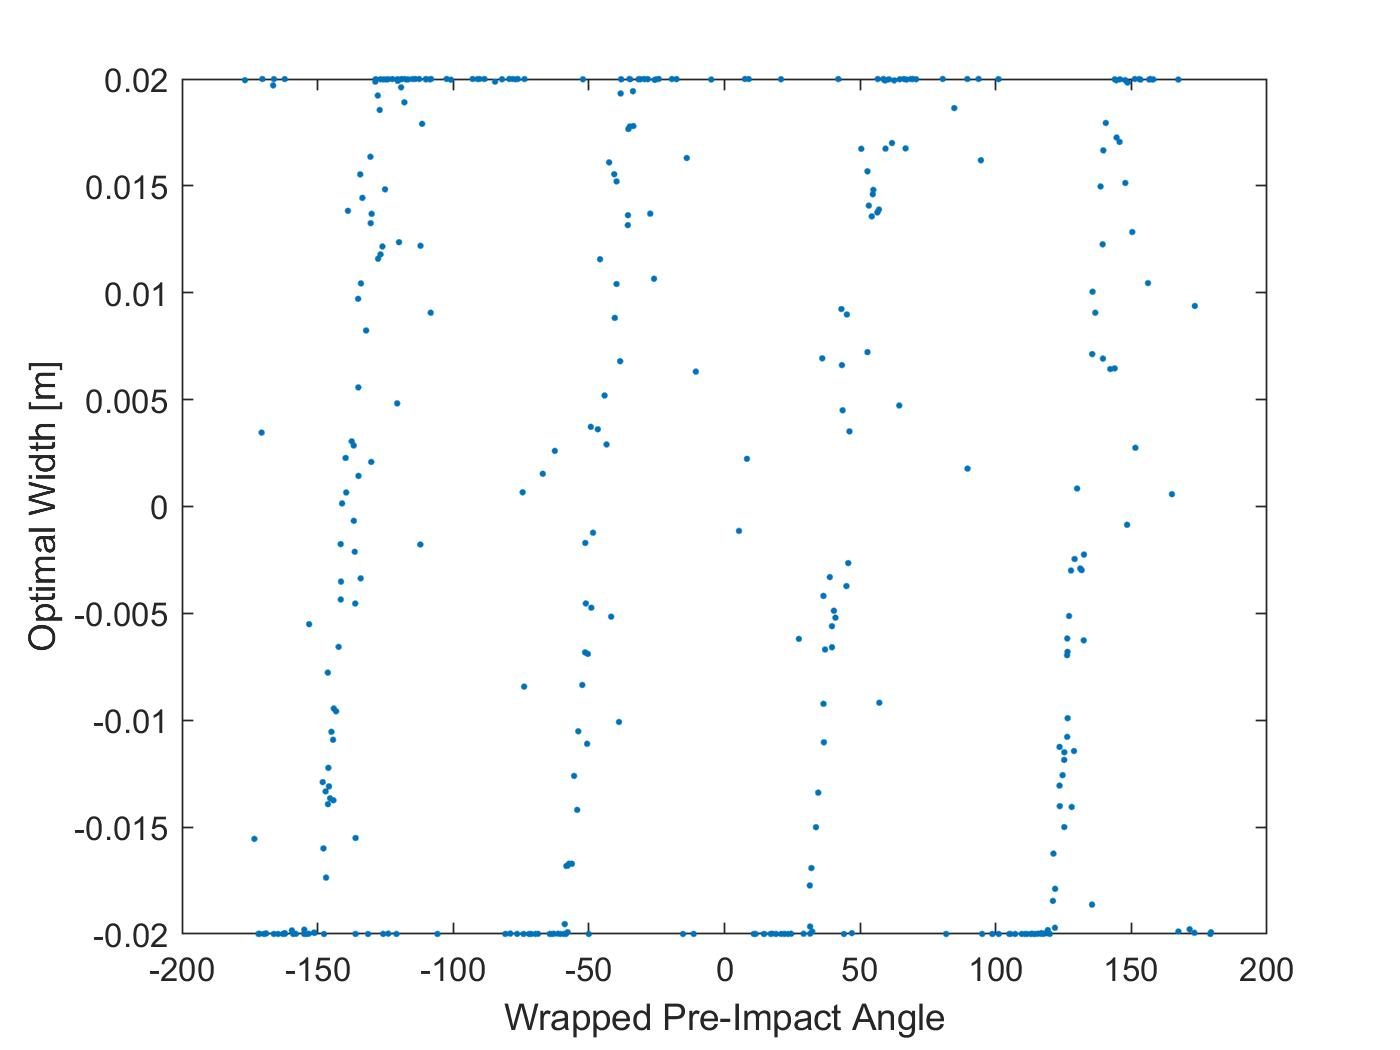
\includegraphics[scale=0.125]{squareAngleWidth.jpg}
        \caption{Square Data Set}
        \label{fig:squareAngleWidth}
    \end{subfigure}
    \caption{Pre-impact Angle vs. Optimal Width for IRB Model (Capped at 2cm)}
\end{figure}

\section{More Angle Exploration}
Using the classical IRB model, we found some new trends between the observed change in angular velocity and the error (Fig \ref{fig:changeInOmegaEllipse}). The cases where we observe very high error are primarily when there are small changes in angular velocity. This also comes back to a point discussed last group meeting, where adding a width to reduce error is not due to a lack of moment or an angular velocity prediction that was too small in magnitude. 
\begin{figure}[h!]
    \centering
    
     \begin{subfigure}[b]{0.45\linewidth}
            \centering
            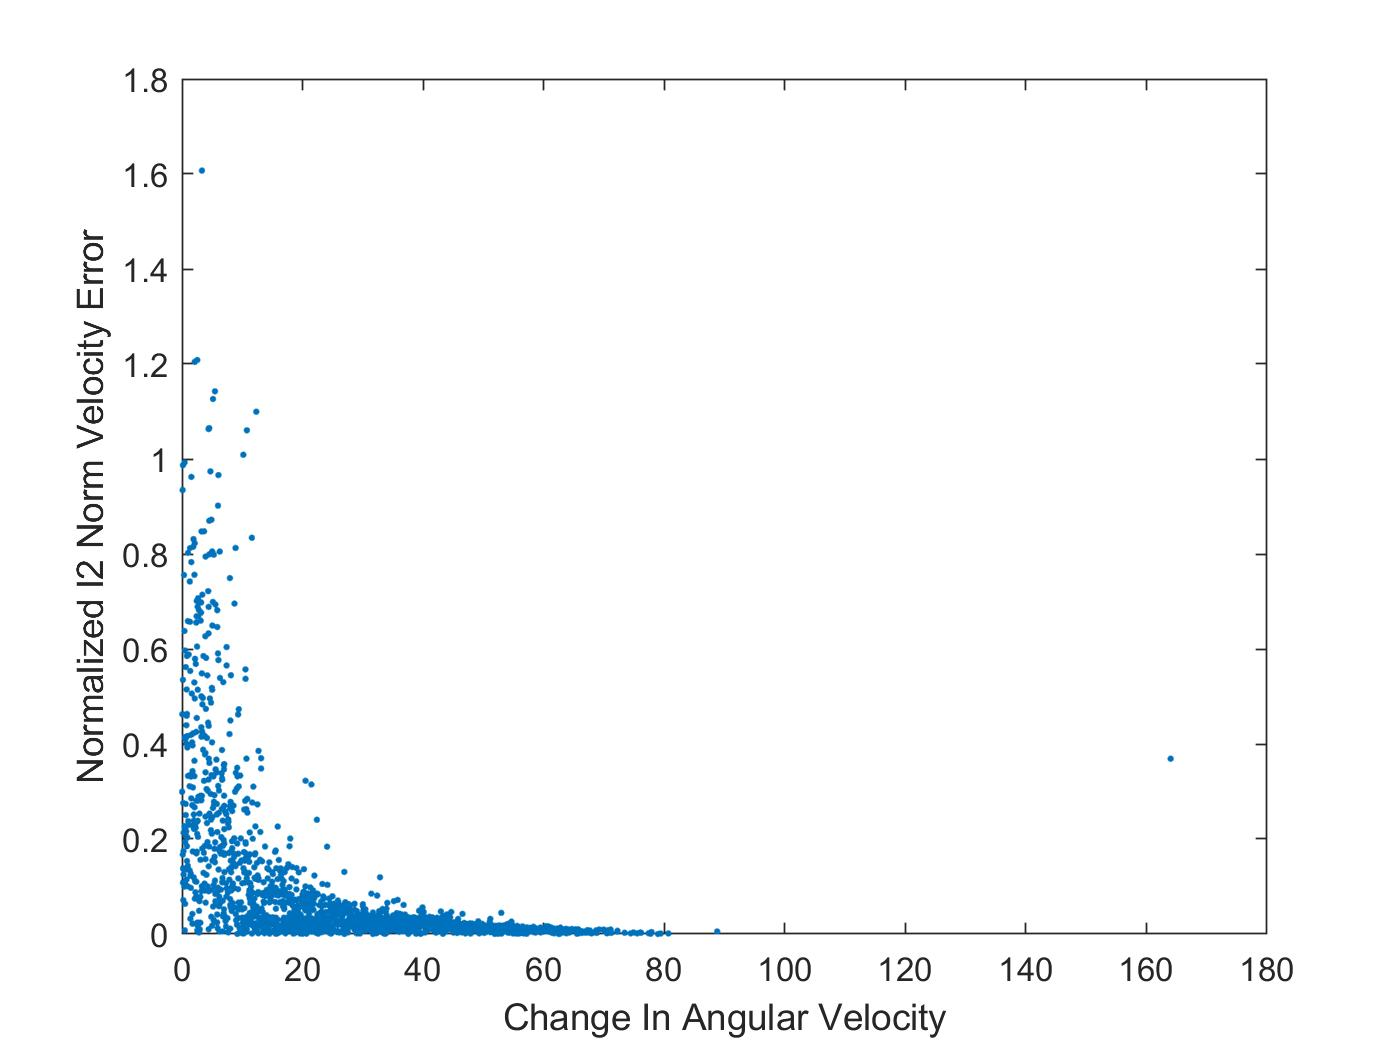
\includegraphics[scale=0.12]{changeInOmegaEllipse.jpg}
            \caption{Ellipse Data Set}
            \label{fig:changeInOmegaEllipse}
    \end{subfigure}
    \quad
    \begin{subfigure}[b]{0.45\linewidth}
            \centering
            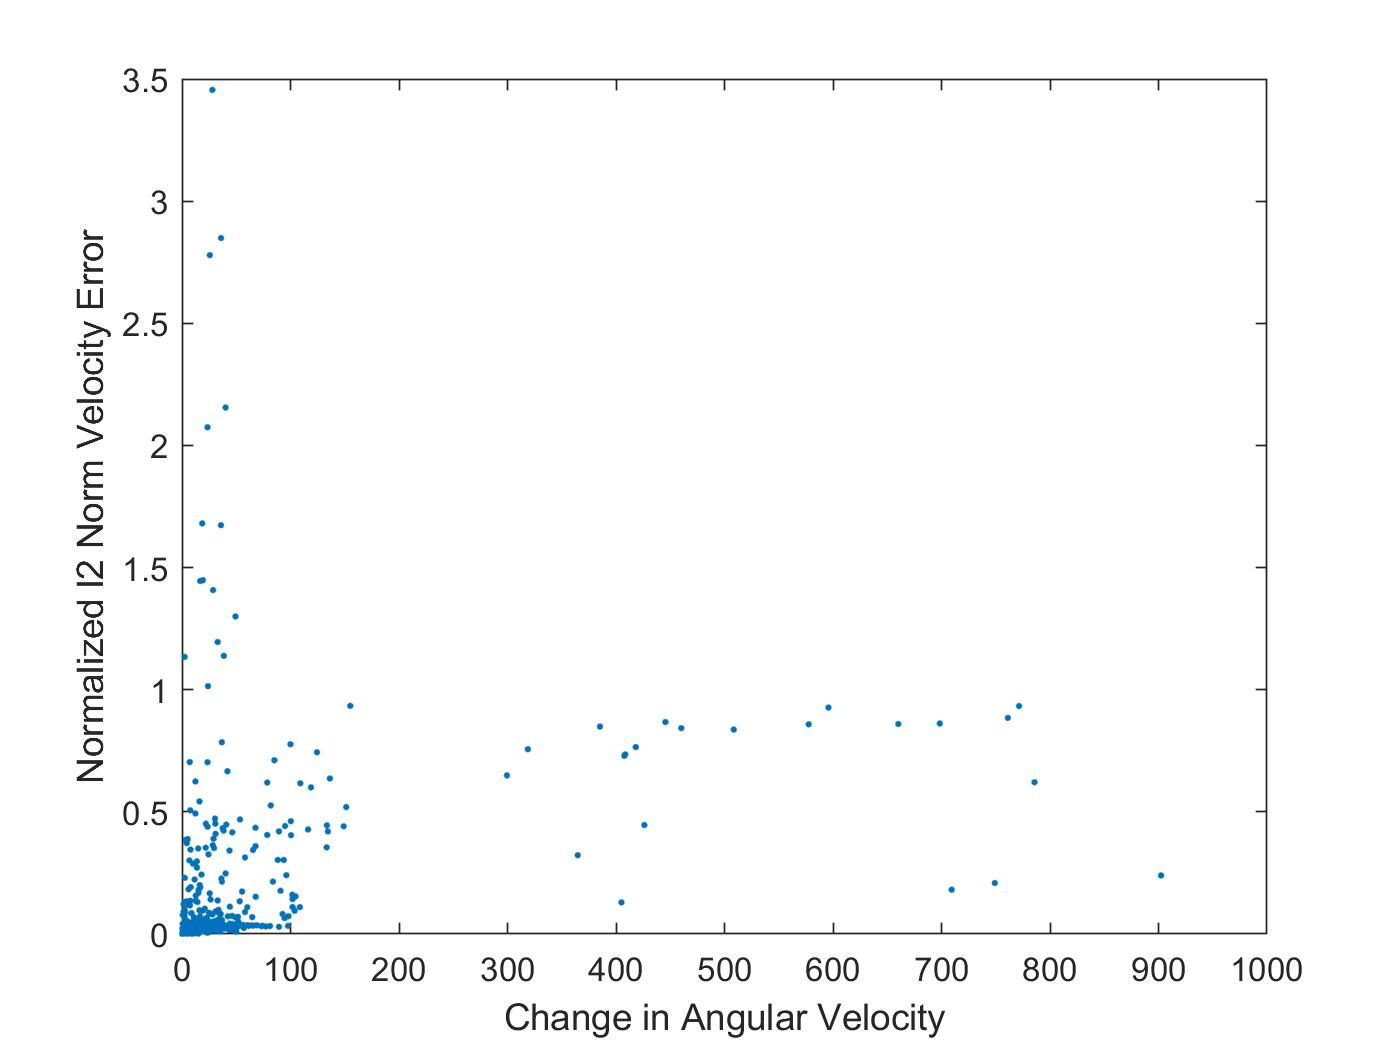
\includegraphics[scale=0.12]{changeInOmegaSquare.jpg}
            \caption{Square Data Set}
            \label{fig:changeInOmegaSquare}
    \end{subfigure}
    \caption{Absolute value of change in angular velocity compared to error from the}
\end{figure}

\noindent A similar trend arises from the square data (Fig \ref{fig:changeInOmegaSquare}), which matches an observation we made when trying to improve our data set. When we first ran the classical IRB model, we looked for outliers with extremely high error to re-watch on the visualizer and double check that we hadn't made any mistakes in labeling the impacts. Sometimes it turned out that the high error was due to a double impact we had mis-categorized and resulted in a removal of that data point, but other times, it was when the square would land on the corner, and just bounce straight up with an angular velocity of around zero.

\newpage
\section{More Square Data Exploration}
After selecting manually selecting our data from the Square Data set as outlined above, we went out to try and replicate some of the patterns we were seeing with the ellipse data. In the plots below, we can observe these patterns:  

\begin{figure}[h!]
     \begin{subfigure}[b]{0.45\linewidth}
            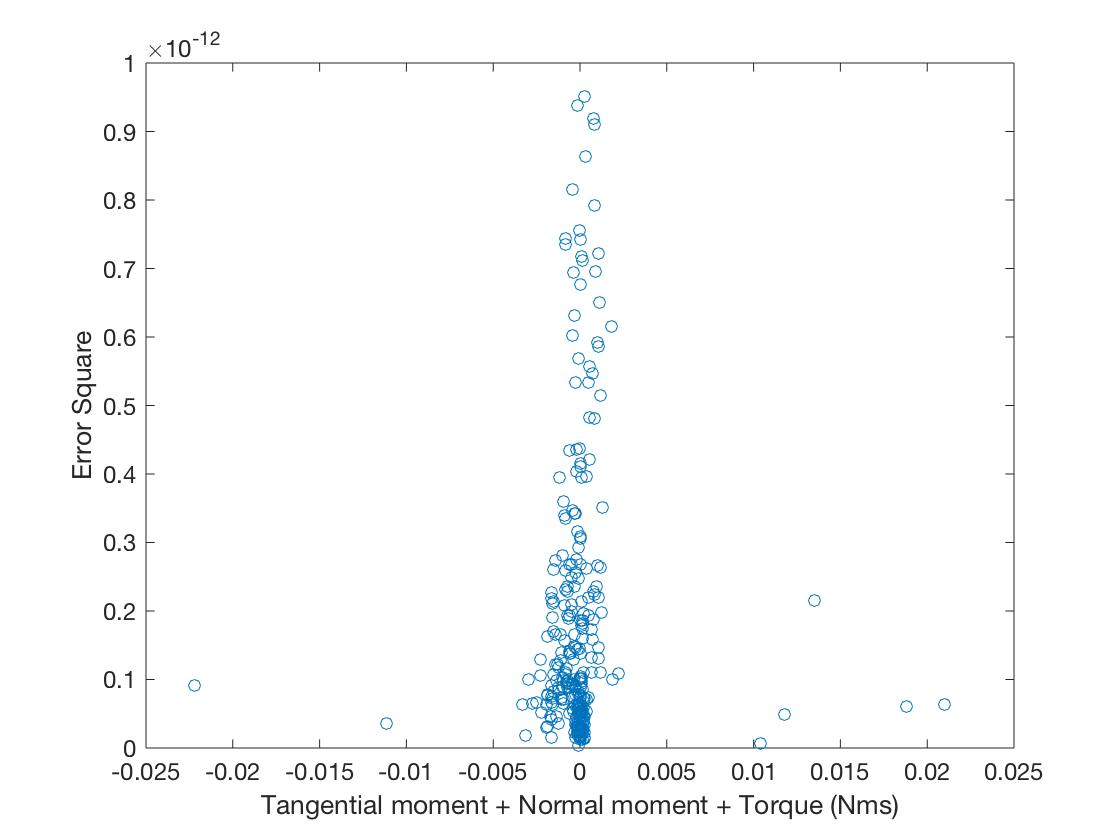
\includegraphics[scale=0.15]{SquarePlot11.jpg}
            \caption{Net Moment vs Error Square}
    \end{subfigure}
    \quad
    \begin{subfigure}[b]{0.45\linewidth}
            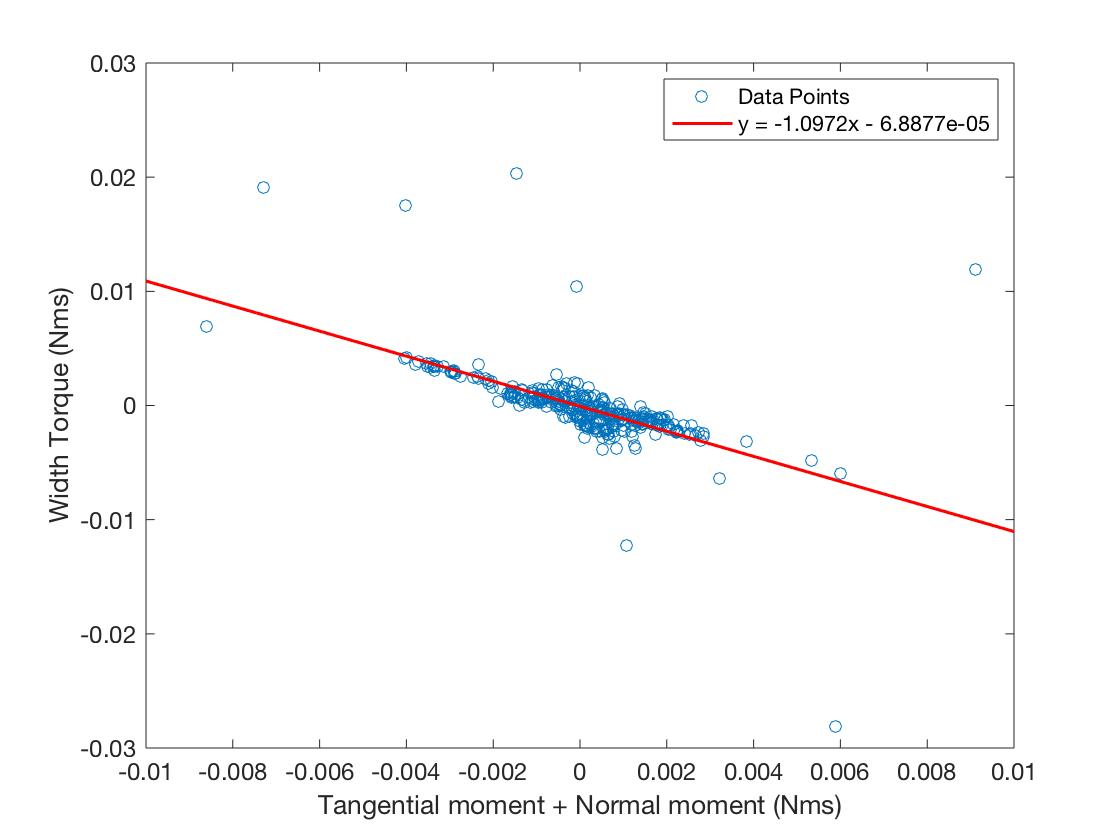
\includegraphics[scale=0.15]{SquarePlot22.jpg}
            \caption{IRB moment vs Width Torque}
    \end{subfigure}
\end{figure}


\end{document}
